\documentclass[12pt]{article}
\def\name{Suruz Miah}
\def\grantName{TeeJet Adaptive Controls Research Project~--~2020}
\def\proposalTitle{Model-Free Adaptive Flow Rate Control of Heterogeneous Agricultural
  Spraying Machines}


\def\dept{Electrical and Computer Engineering Department}
\def\college{Caterpillar College of Engineering and Technology}
\def\uName{Bradley University}

\usepackage[utf8]{inputenc}
\usepackage[dvipsnames]{xcolor}
\oddsidemargin=-0.2in % -.3 for a4 paper
\evensidemargin=.5in
\textwidth=7.0in
\topmargin=-0.5in
\textheight=9.0in
\parindent=.2in
\newcommand{\vsmallskip}[0]{}
\newcommand{\midskip}[0]{\vspace{3mm}}
\newcommand\todoin[2][]{\todo[inline, caption={2do}, #1]{ \begin{minipage}{\textwidth-4pt}#2\end{minipage}}}


\usepackage{fancyhdr,lastpage}
\usepackage{hyperref}
\hypersetup{
    % pdfmenubar=true,        % show Acrobat’s menu?
    % pdffitwindow=false,     % window fit to page when opened
    % pdfstartview={FitH},    % fits the width of the page to the window
    % pdfnewwindow=true,      % links in new window
    colorlinks=true,       % false: boxed links; true: colored links
    linkcolor=blue,          % color of internal links
    citecolor=red,        % color of links to bibliography
    filecolor=magenta,      % color of file links
    urlcolor=blue           % color of external links
  }
  
\usepackage{amsmath,amssymb,bm}
\usepackage{graphicx}
\usepackage{rotating}
% \epstopdfsetup{suffix=}
\usepackage[nottoc,notlot,notlof]{tocbibind} % include References in table of contents
%\usepackage[table,usenames,dvipsnames]{xcolor}
\usepackage{xtab}
\usepackage{siunitx}
\sisetup{unitsep=\cdot}
\usepackage{setspace}
\usepackage{float}
\usepackage{pdfpages}
\usepackage[english,algo2e,algoruled,vlined,linesnumbered]{algorithm2e}   % package for algorithm
\usepackage{booktabs}
\usepackage[colorinlistoftodos]{todonotes}
\usepackage{pgfgantt} % package for gantt chart
\usepackage{easyReview}
\usepackage{enumerate}

\usepackage{tikz}
% load libraries
\usetikzlibrary{backgrounds,calc,patterns,decorations.pathmorphing,decorations.markings,shapes,arrows,snakes,tikzmark}
\usepackage[siunitx,smartlabels]{circuitikz}
\def\smgrid{0.5}


% %% For Preview-latex using C-c C-p  commands. 
% \usepackage[active,displaymath,sections,graphics,floats]{preview}
% % \usepackage[active,displaymath,textmath,sections,graphics,floats]{preview}
% \PreviewEnvironment{enumerate}  % enumerate environment in the preview
% \PreviewEnvironment{tikzpicture} % tikzpicture in the preview 


%\doublespacing
%\onehalfspacing
\title{\proposalTitle}

%\title{Time--Invariant Partially-Observed Feedback Control Operator for a Class of Uncertain Nonlinear Systems}
%\author{Suruz Miah\thanks{Suruz Miah is with the Electrical and Computer Engineering Department of Bradley University, Peoria, IL, 61625, USA. E-mail: \href{mailto:smiah@bradley.edu}{smiah@bradley.edu}, phone: +1 (306) 677--2260}
%}


\renewcommand{\headrulewidth}{1.5pt}
\renewcommand{\footrulewidth}{0.4pt}

\lhead{S.~Miah,~K.~Vonckx}
\chead{ECE Department}
\rhead{\uName}

\cfoot{%\hspace{\footpageshift}%
       \parbox{4in}{\, \hfill Page~ %
                    \arabic{page} of \protect\pageref*{LastPage} % +LP
%                    \arabic{page}                               % -LP
                    \hfill \,}}
%\lfoot{\grantName}   % header at lower left corner
\lfoot{Application Data Management}   % header at lower left corner
\rfoot{Control System Technology}   % header at lower right corner


\begin{document}
\centerline{\href{http://www.bradley.edu}{
\includegraphics[height=0.5in]{figs/logoBU1-Print}}\hfill\href{https://www.teejet.com/}{
\includegraphics[height=1.0in]{figs/TeeJet-Logo}}}

\begin{center}
\vspace*{1.0cm}
{\LARGE \grantName}


\vspace*{0.25cm}

{\LARGE \textsc{Project Statement}}

\vspace*{0.5cm}

% \normalsize
% Thesis submitted to the\\
% Faculty of Graduate and Postdoctoral Studies\\
% In partial fulfillment of the requirements\\
% For the degree \degreePhD~ in\\
% \nameofprogram\\
\vspace*{1.5cm}
{\color{BrickRed}
\hrule height 1.5pt
\midskip
}
%\begin{flushleft}
{\LARGE 
% \textsc{Title:} 
\proposalTitle
}
%\end{flushleft}
\midskip
{\color{BrickRed}
\hrule height 1.5pt
\midskip
}
\vspace*{0.01cm}
\begin{flushright}
{\large
 Principal Investigator (PI):  Dr.~\href{http://personalpages.bradley.edu/~smiah}{Suruz \textsc{Miah}}\\
 Research Partner: Ken \textsc{Vonckx}, TeeJet Technology
  % Technical Adviser: Dr. Kaisar R.  \textsc{Khan}\\  
}
\end{flushright}

\vspace*{1.0cm}
\begin{flushleft}
{\color{BrickRed}
{\Large \textsc{Contact Information}}\\
\vskip10pt
\hrule height 1pt
\midskip
}
\vskip10pt
Dr. Suruz Miah\\
Assistant Professor\\
\dept\\
\college\\
\href{http://www.bradley.edu/}{\uName}\\
\vskip10pt
Business and Engineering Convergence Center \#4269 \\
1501 W. Bradley Avenue\\
Peoria, IL, 61625, USA\\
\vskip10pt
Phone:~+1 (309) 677--2260\\
e-Mail:~\href{mailto:smiah@bradley.edu}{smiah@bradley.edu}\\
Website:~\href{http://personalpages.bradley.edu/~smiah/}{http://personalpages.bradley.edu/\~~smiah/}
\vskip15pt
\end{flushleft}

\end{center}
\thispagestyle{empty}
\newpage

%\date{ }
%\maketitle
%
%\thispagestyle{fancy} % shows header and footer on all the  pages (including first page)
%\thispagestyle{empty}
\pagestyle{fancy}

 \renewcommand{\contentsname}{Table of Contents}
 \tableofcontents 
 \listoffigures
 
\newpage

\section*{List of Abbreviations}
\label{sec:abbreviations}
\addcontentsline{toc}{section}{List of Abbreviations}

\begin{tabular}{ll}
  {\bf PWM}& Pulse Width Modulation\\
\end{tabular}
\section{Background}
\label{sec:background}

Agricultural Spraying machines are used to apply chemical to farmland to increase the productivity of the land.  Fertilizer increases yield by $40\%$ to $60\%.$  If pesticides are not used, yield decreases by $50\%$ to $90\%.$  To maximize these yields, the correct amount of chemical must be applied to the correct area of the \replace{plat}{plant} or soil. \add{Chemical is applied using sprayers which are connected to a pump through plumbing system. A two-way plumbing diagram of an agricultural spraying machine is shown in Figure~\ref{fig:twoWayPlumbingDiagramSrayingMachine}\todo{Illustrate this figure}.}
%
\begin{figure}
  \centering
  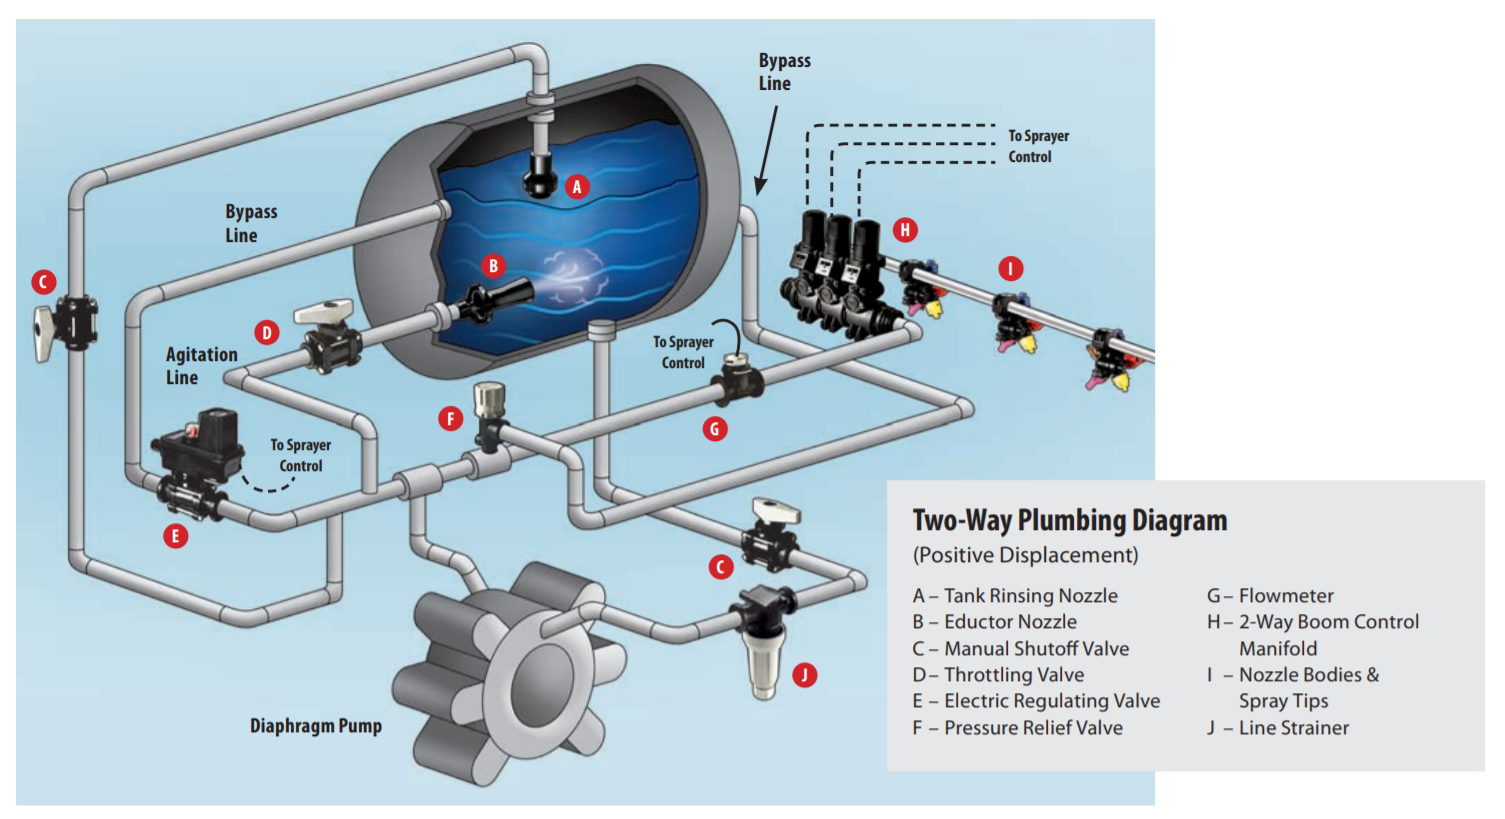
\includegraphics[width=0.7\textwidth]{figs/img/twoWayPlumbingDiagramSrayingMachine}
  \caption{Two-way plumbing diagram of an agricultural srayping machine [Courtesy of TeeJet Technologies].}
  \label{fig:twoWayPlumbingDiagramSrayingMachine}
\end{figure}



\section{Problem Statement and Objectives}
\label{sec:probl-stat-object}

All sprayers have a pump that forces chemical from a tank through hydraulic plumbing leading to the boom of the sprayer \add{(see Figure~\ref{fig:twoWayPlumbingDiagramSrayingMachine})}.  Flow to the boom can be changed by either changing the speed of the pump or by opening and closing a regulation valve.

Across the boom are a number of nozzles that serve as the exit point for fluid.  These nozzles also have a solenoid that can open or close the valve.  By applying a PWM signal, we can \todo{$\ldots$ continue} When spaying, the farmer is limited to how fast he/she can drive and apply the correct amount of chemical without increase. In a sprayer application, we have two separate discrete-time feedback control systems to solve these problems.

\begin{enumerate}
\item One system controls to a desired flow rate.  This system ensures the correct amount of fluid is applied to the field.  Target flow is calculated by the prescription for the field and the speed of the vehicle. 

\item A second system controls to a constant pressure across the boom of a sprayer.  Droplet size directly correlates to pressure and can be determined from the nozzle’s datasheet.  This ensures proper application of the fluid and prevents drift due to atmospheric conditions.  

\end{enumerate}

Flow rate controllers, pressure controllers, and sprayers can all be manufactured by  different companies.  This makes it very difficult to come up 
with a design that will \replace{preform}{perform} well across different
scenarios.  \add{Figure~\ref{fig:twoInputTwoOutputDT-ControlSystem} shows the
  block diagram of a two-input two-output discrete-time control system block
  diagram, where  $D_2(z),$ $G(z),$ $x_2^{[d]},$ and $x_2$ are assumed to be
  unknown.} %
%

\begin{figure}
  \centering
  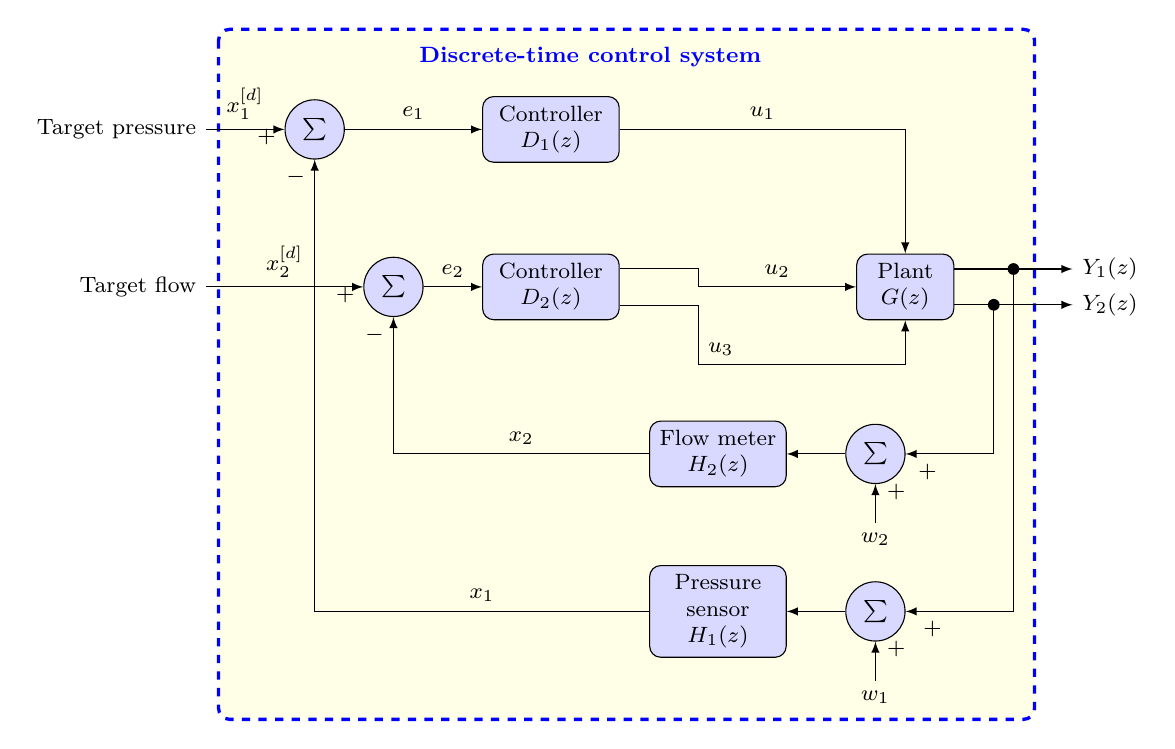
\begin{tikzpicture}    
      \tikzstyle{every node} = [font=\footnotesize]
      \tikzstyle{block} = [draw, rectangle, fill=blue!15, rounded corners, minimum height=0.5 cm, minimum width=1.0 cm]
      \tikzstyle{sum} = [draw, circle, fill=blue!15];
      \tikzstyle{pinstyle} = [pin edge={to-,thin,black}]
      % Place nodes
      \node[sum](sum){$\sum$};
      \node[block, text width=1.5 cm, text centered, right of = sum, node distance=3 cm](D1){Controller $D_1(z)$};
      \node[block, text width=1.5 cm, text centered, below of = D1, node distance=2 cm](D2){Controller $D_2(z)$};
      \node[sum, left of = D2, node distance=2.0 cm](sum3){$\sum$};
      \node[block, text width=1 cm, text centered, right of = D2, node distance=4.5 cm](G){Plant $G(z)$};      
      \node[block, text width=1.5 cm, text centered, below right of = D2, node distance=3.0 cm](H2){Flow meter $H_2(z)$};
      \node[block, text width=1.5 cm, text centered, below of = H2, node distance=2.0 cm](H1){Pressure sensor $H_1(z)$};
      \node[sum, right of = H2, node distance=2 cm](sum2){$\sum$};
      \node[sum, right of = H1, node distance=2 cm](sum1){$\sum$};      

      % Connections 
      \draw[latex-]
      (sum.west)-- node[midway,above]{$x_1^{[d]}$}++(-2*\smgrid,0)node[anchor=east]{Target pressure};
      \draw
      (sum.-165)node[left]{$+$};
      \draw[latex-]
      (sum3.west)-- node[midway,above]{$x_2^{[d]}$}++(-4*\smgrid,0)node[anchor=east]{Target flow};
      \draw
      (sum3.-165)node[left]{$+$};
      
      \draw[-latex]
      (sum.east) -- node[midway,above]{$e_1$}(D1.west);
      \draw[-latex]
      (sum3.east) -- node[midway,above]{$e_2$}(D2.west);
      \draw[-latex]
      (D1.east) -| node[near start,above]{$u_1$} (G.north);
      \draw[-latex]
      (D2.15) --++(2*\smgrid,0)|- node[near end,above]{$u_2$}(G.west);
      \draw[-latex]
      (D2.-15) -|node[very near end,right]{$u_3$}++(2*\smgrid,-1.5*\smgrid)-| (G.south);

      \draw[-latex]
      (G.20) -- ++(3*\smgrid,0)node[above,right]{$Y_1(z)$};
      \draw[-latex]
      (G.-20) -- ++(3*\smgrid,0)node[below,right]{$Y_2(z)$};
      \draw[-latex]
      ($(G.20) + (1.5*\smgrid,0)$)node[fill,circle,inner sep=1.5pt]{} |- (sum1.east)node[very near end,below]{$+$};
      \draw[-latex]
      ($(G.-20) + (\smgrid,0)$)node[fill,circle,inner sep=1.5pt]{} |- (sum2.east)node[very near end,below]{$+$};

      \draw[-latex]
      (sum2.west) -- (H2.east);
      \draw[-latex]
      (H2.west) -| node[near start,above]{$x_2$} (sum3.south)node[anchor=north east]{$-$}; 
      
      \draw[-latex]
      (sum1.west) -- (H1.east);
      \draw[-latex]
      (H1.west) -|node[near start,above]{$x_1$} (sum.south)node[anchor=north east]{$-$}; 

      \draw[latex-]
      (sum2.south) -- ++(0,-\smgrid)node[below]{$w_2$};
      \draw
      ($(sum2.-90)+(0.05*\smgrid,-0.2*\smgrid)$)node[below,right]{$+$};
      \draw[latex-]
      (sum1.south) -- ++(0,-\smgrid)node[below]{$w_1$};
      \draw
      ($(sum1.-90)+(0.05*\smgrid,-0.2*\smgrid)$)node[below,right]{$+$};
      
      % Layers
      \begin{pgfonlayer}{background}
        \filldraw[fill=yellow!10,draw = blue,dashed,very thick, rounded corners]
        ($(sum.north west) + (-1.9*\smgrid,2*\smgrid)$) rectangle ($(sum1.south east)+(3.5*\smgrid,-2.2*\smgrid)$);
      \end{pgfonlayer}
      \draw
      ($(D1.north)+(\smgrid,\smgrid)$)node[]{\textcolor{blue}{{\bf Discrete-time control system}}};
    \end{tikzpicture}  
  \caption[Two-input, two-output discrete-time control system block diagram.]{Two-input, two-output discrete-time control system block diagram.}
  \label{fig:twoInputTwoOutputDT-ControlSystem}
\end{figure}
%
\begin{table}
  \centering
  \caption{Description of signals used in the control system block diagram shown in Figure~\ref{fig:twoInputTwoOutputDT-ControlSystem}.}
  \label{tab:signalDescription}
  \begin{tabular}{ll}
    \toprule[1.5pt]
    Signal& Description\\
    \toprule
    $x_1^{[d]}$ & Target pressure\\
    $x_2^{[d]}$ & Target flow\\
    $x_1$ & Actual pressure\\
    $x_2$ & Actual flow\\
    $D_1(z)$ & Pressure controller \add{transfer function}\\
    $D_2(z)$ & Flow controller \add{transfer function}\\
    $u_1$ & Duty cycle to solenoids (limited between $0$ and $100$)\\
    $u_2$ & Open/close signal for regulating valve\\
    $u_3$ & Pump speed (optional)\\
    $G(z)$ & Plant model\\
    $H_1(z)$ & Pressure sensor model (transfer function)\\
    $H_2(z)$ & Flow meter model (transfer function)\\
    $w_1$ & Pressure sensor noise\\
    $w_2$ & Flow meter noise\\
    \bottomrule[1.5pt]
  \end{tabular}
\end{table}
%

{\bf Problem statement:} Develop a control system that can adapt to different plant models and \comment{rate controllers.}{Do you mean flow rate and target pressure controllers?}

{\bf Outcomes:}

\textit{TeeJet} expects design of a  control system that can adapt to: %
\begin{enumerate}
\item Different plant models
  
\item Different rate controllers 
\end{enumerate}

\textit{Student experience}  are expected to learn the following items that pertain to proposed control system:
\begin{enumerate}
\item Design the control system that is ready for implementation
  
\item Conduct computer simulations using MATLAB and Simulink
  
\item Validation and testing using real-time embedded system 
  

\end{enumerate}


\section{Solution Approach}
\label{sec:solutionApproach}

Model-Free Reinforcement Learning Control Approach


\section{Deliverables}
\label{sec:deliverables}

TBD

\section{Timeline and Milestones}
\label{sec:timeline}



% %
\begin{figure}
  % \begin{sidewaysfigure}
    \centering
    \begin{ganttchart}[hgrid,
      vgrid={*8{black, dotted},*8{black,dotted},*8{black, dotted},*8{black,dotted}},
      title/.style={fill=gray!15,draw=black},
    group/.append style={draw=black, fill=yellow!50},
    group left shift = 0,
    group right shift = 0,
    x unit=.5cm,  % Controls the x-axis grid width of the chart
    y unit title=.8cm,
    y unit chart=.6cm,
    milestone label font=\tiny,
    bar label font=\small, 
    group label font=\normalsize,
    bar/.append style={draw=black,fill=blue},
    bar left shift= 0,
    bar right shift= 0,
    bar height = .7]{1}{20}  % Total number of weeks, from 1 to 20, for example 
    \gantttitle{2020}{20}  % Number of weeks in 2020 
    % \gantttitle{2021}{16}    % Number of weeks in 2021 
    \\
    \gantttitle{July}{4}
    \gantttitle{Aug}{4}
    \gantttitle{Sep}{4}
    \gantttitle{Oct}{4}
    \gantttitle{Nov}{4}\\
    \ganttgroup[progress=25]{{\bf Problem description}}{1}{4}\\
    \ganttbar{Problem analysis}{1}{2}\\
    \ganttbar{Deliverables}{2}{4}\\
%    
    \ganttgroup[progress=25]{{\bf Solution approach}}{2}{8}\\
    \ganttbar{Model-free analysis}{3}{5}\\
    \ganttbar{Reinforcement learning setup}{4}{8}\\
    \ganttgroup[progress=0]{{\bf Implementation}}{8}{16}\\
    \ganttbar{Matlab simulation}{8}{10}\\
    \ganttbar{Simulink implementation}{8}{12}\\
    \ganttbar{Embedded system implementation}{10}{16}\\
    \ganttgroup[progress=0]{{\bf Publication/report}}{16}{20}\\
    \ganttbar{Conference/journal paper}{16}{18}\\
    \ganttbar{Report/workshop/presentation}{16}{20}
  \end{ganttchart}
\caption{Gantt chart showing the project activities from July 2020 to November 2020.}
\label{fig:gantt1}
% \end{sidewaysfigure}
\end{figure}

  
% \end{itemize}
% %
% 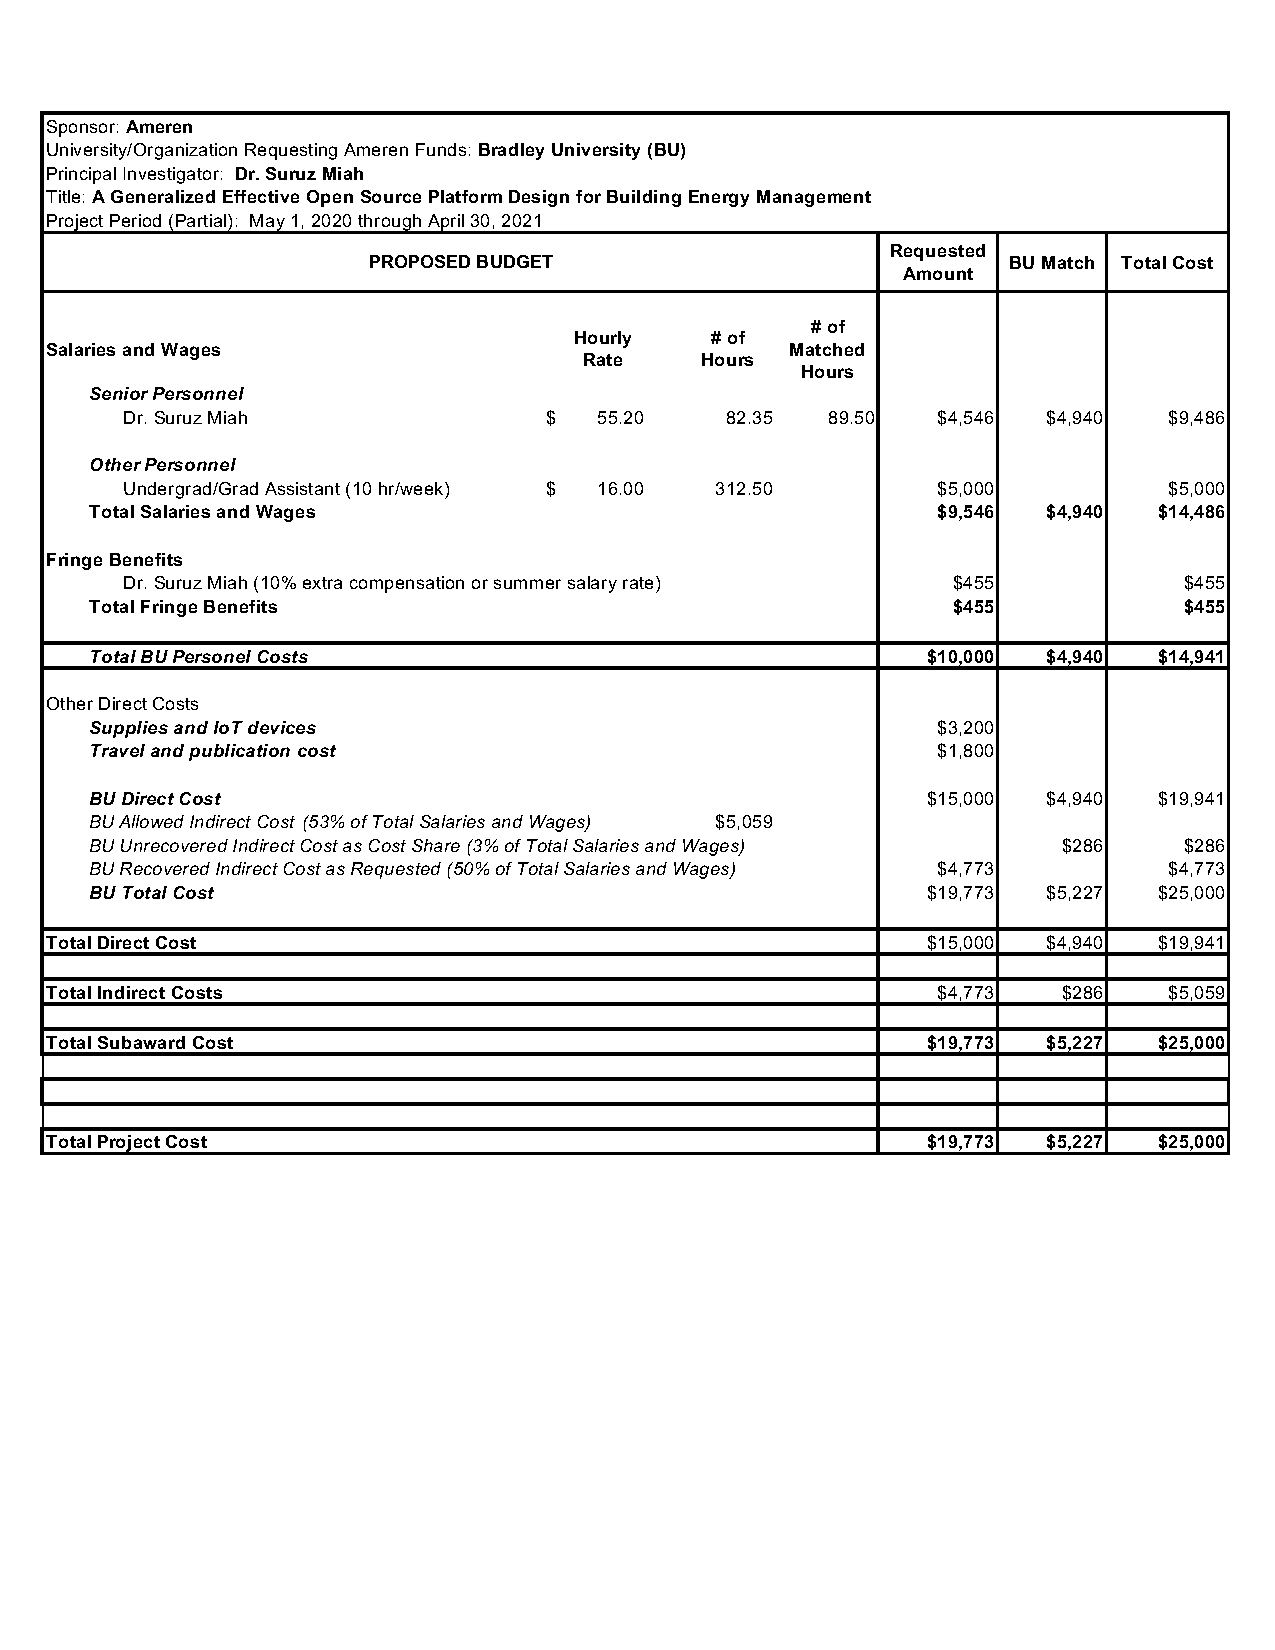
\includepdf[pagecommand={\thispagestyle{fancy}}]{supportingDocs/seedGrantBEMS-AmerenV1.pdf}      

% \subsection{Biographical Sketch of PI}
% PI's biographical sketch is attached in the next page. 
% \includepdf[pages=-,pagecommand={\pagestyle{fancy}}]{supportingDocs/bioSketchMiah.pdf}



%%% Local Variables:
%%% mode: latex
%%% TeX-master: "../mainProposal"
%%% End:


\bibliographystyle{IEEEtran}
\bibliography{bib/refsEnergy.bib,bib/refsSuruzWeb}
\end{document}



%%% Local Variables:
%%% mode: latex
%%% TeX-master: t
%%% End:
